\documentclass[10pt]{article}
\usepackage[preprint]{tmlr}
\usepackage{amsmath,amssymb,booktabs,graphicx,hyperref,url}
\hypersetup{pdfauthor={Goutham Siripuram},pdftitle={Question-Only Selection of Bounded Reasoning Workflows: Baselines, Budget Transfer, and a Local Evaluation}}
\title{Question-Only Selection of Bounded Reasoning Workflows: Baselines, Budget Transfer, and a Local Evaluation}
\author{\name Goutham Siripuram}
\begin{document}
\maketitle
\begingroup\renewcommand{\thefootnote}{}\footnotetext{Generative AI assisted drafting, code development, editing, and internal technical validation. The human author is responsible for the manuscript and its scientific claims. This assistance is not independent peer review.}\endgroup
\begin{abstract}
Choosing a reasoning workflow from a question requires evidence that selection improves on a simpler fixed policy. We evaluate a question-only ridge baseline against a training-selected constant workflow using two local checkpoints, four workflows, two seeds, separate GSM8K training and test cohorts, and SVAMP transfer questions. The 4,096 recorded executions include a larger output-allowance condition on GSM8K. At the primary 512-token allowance, router-minus-constant utility is -0.00894 for Qwen3 and -0.04075 for Qwen2.5; the study does not establish a consistent routing advantage. A separately specified parsing heuristic also changes the interpretation of Qwen2.5 workflow rankings. The contribution is a constrained negative evaluation with explicit training isolation, budget transfer, and scoring sensitivity, rather than a new routing algorithm. The results motivate checking simple baselines and outcome definitions before attributing gains to workflow selection.
\end{abstract}
\section{Introduction}
A workflow selector adds a learned decision to an already stochastic inference process. Its value cannot be inferred from the best workflow observed after evaluating a question: a deployable selector must choose using information available beforehand. This study asks whether six question-derived features and a simple training-only predictor outperform one workflow selected from the same training data.

The contribution is an evaluation of this constrained baseline under two forms of transfer: a larger output allowance and a different arithmetic benchmark. It also examines whether conclusions depend on strict response formatting. The results are primarily negative for routing, and they expose a substantial scoring discrepancy for one checkpoint. We do not present ridge regression or adaptive workflow selection as new algorithms.

Researchers and system builders can use the released protocol to distinguish a deployable selection gain from hindsight selection, and to check whether a reported architectural ranking survives a separately stated scorer. The experiment does not demonstrate monetary savings or improved production deployments. Its practical value is a reproducible caution about baseline choice and what the measured outcome represents.

\section{Related work}
OneFlow examines strong single-agent implementations of homogeneous workflows, including context and cache considerations \citep{xu2026oneflow}. Budget-aware comparisons also emphasize context and computation as confounders \citep{tran2026equalbudget}. Our token ceilings do not equalize actual input context, generation length, or compute, and we make no causal claim about agent count alone.

CB-Orchestrator combines workflow-pool construction with contextual-bandit selection based on query and workflow representations \citep{sun2026cborchestrator}. Our four fixed workflows, exhaustive training outcomes, lexical features, and ridge predictors are a substantially simpler baseline. We do not implement that system, so negative results here neither refute its findings nor establish competitive performance against it. The absence of stronger learned selectors is a limitation.

GSM8K supplies the training and held-out test cohorts \citep{cobbe2021gsm8k}; SVAMP supplies the transfer cohort \citep{patel2021svamp}. SVAMP was constructed through variations of existing word problems. Both datasets concern arithmetic, so transfer between them is narrower than generalization to unrelated domains.

% Manuscript fragment describing the frozen analysis, not completed results.
\section{Selection from question-only information}
\label{sec:selection-formulation}
Let $\mathcal W$ contain the four specified workflows and let $q$ be a question.
For checkpoint $h$, workflow $w$, seed $s$, and output allowance $B$, write
$Y_{h,q,w,s,B}\in\{0,1\}$ for format-constrained exact-answer success and
$T_{h,q,w,s,B}$ for generated tokens. The declared utility is
\begin{equation}
 U_{h,q,w,s,B}^{(\lambda)}
 =Y_{h,q,w,s,B}-\lambda T_{h,q,w,s,B}/B.
 \label{eq:workflow-utility}
\end{equation}
For $\lambda\geq0$ and a valid execution within budget, this utility lies in
$[-\lambda,1]$. The penalty is a chosen exchange rate, not a measured monetary
cost. In particular, dividing by $B$ means a token has a different penalty at
different allowances. Comparisons at 512 and 1,024 tokens therefore describe
performance under their respective normalized utilities; they are not a
fixed-price economic comparison across budgets.

\subsection{Training and deployment rules}
For each checkpoint and penalty, average utility across the two seeds of each
training question to obtain $\bar U_{q,w}^{(\lambda)}$. Let $z(q)$ contain the
six frozen question features after training-set standardization, and let
$d(q)=(1,z(q)^\top)^\top$. Each workflow receives a ridge predictor,
\begin{equation}
 \widehat\beta_w=\mathop{\mathrm{argmin}}_{\beta}
 \sum_{q\in\mathcal D_{\mathrm{train}}}
 (\bar U_{q,w}^{(\lambda)}-d(q)^\top\beta)^2
 +\sum_{k=1}^{6}\beta_k^2.
 \label{eq:ridge-router}
\end{equation}
The intercept $\beta_0$ is unpenalized. All targets use the 512-token training
condition, and the penalty on coefficients is fixed rather than tuned on
evaluation data. Prediction selects
$\pi(q)=\mathrm{argmax}_{w\in\mathcal W}d(q)^\top\widehat\beta_w$.
The fixed workflow order resolves ties. This is a transparent baseline, not
a new optimization algorithm.

The training-selected constant $w_0$ maximizes average utility over the same
training questions. On an evaluation cohort $\mathcal D$, the primary contrast
is
\begin{equation}
 \widehat D=\frac{1}{|\mathcal D|}\sum_{q\in\mathcal D}
 \left(\bar U_{q,\pi(q)}^{(\lambda)}-
       \bar U_{q,w_0}^{(\lambda)}\right).
 \label{eq:router-contrast}
\end{equation}
Both policies are fixed before inspecting evaluation outcomes. The two-seed
average is the evaluation unit within a question; uncertainty resamples
questions and retains paired workflow outcomes. The resulting intervals
condition on the fitted policies rather than incorporating new-training-sample
variation. The 1,024-token test condition and SVAMP cohort do not refit either
policy.

\subsection{A descriptive hindsight reference}
The analysis also records
\begin{equation}
 \widehat R_{\mathrm{obs}}(\pi)=
 \frac{1}{|\mathcal D|}\sum_{q\in\mathcal D}
 \left(\max_{w\in\mathcal W}\bar U_{q,w}^{(\lambda)}
       -\bar U_{q,\pi(q)}^{(\lambda)}\right).
 \label{eq:observed-oracle}
\end{equation}
This reference chooses a different workflow for each question using that
question's observed two-seed outcomes. It is neither the best single constant
on the test set nor a deployable selector. Its nonnegative value follows from
the pointwise maximum, not from a guarantee about true expected utility.
Selecting from noisy observed outcomes makes this a deliberately optimistic
hindsight reference. It cannot establish attainable gains from question-only
routing.

For the alternative parsing heuristic, the primary policy choices remain
unchanged and the same executions are rescored. A discrepancy between scoring
views concerns the interpretation of the outcome; it does not authorize choosing
the more favorable view as a replacement primary analysis. Budget saturation
and answer-revision transitions are descriptive diagnostics, not additional
proof of an architectural advantage.

\section{Evaluation design}
\subsection{Selection problem}

The decision is which bounded reasoning workflow to execute for a question. The selector observes only the question text. It cannot inspect candidate answers, gold labels, or evaluation outcomes before choosing. The proposed experiment tests a transparent routing baseline rather than a new routing algorithm or a universal claim about agent count.

Four workflows use the same checkpoint in every role: direct solution, solution with self-refinement, plan followed by solution, and plan followed by solution and verification. Role changes alter prompts and information flow. They do not create independent experts. No workflow in this study uses an external tool.

\subsection{Cohorts and inference allowances}

The fixed cohorts comprise 64 GSM8K training questions, 64 different GSM8K test questions, and 64 SVAMP transfer questions. Eight separate GSM8K training questions were reserved for development. Normalized question text excludes overlap with the pilot and the reliability experiment. SVAMP sampling admits at most one item per numeric-masked body group. These exclusions do not eliminate semantic overlap or possible model-pretraining contamination.

Each workflow is evaluated with two seeds using Qwen3-0.6B and Qwen2.5-1.5B-Instruct. All cohorts receive a maximum allowance of 512 generated tokens per workflow. Allocations are 512 for direct solution, 256 plus 256 for self-refinement, 96 plus 416 for planning and solving, and 96 plus 288 plus 128 for planning, solving, and verification. Unused allowance is not transferred between roles. The GSM8K test cohort also has a 1,024-token condition with proportionally doubled allocations. The full design specifies 4,096 workflow records.

The larger allowance was selected during development, before evaluation, in response to intermediate truncation and missing final responses. Equal output ceilings do not equalize realized output, input context, latency, or floating-point computation. Those distinctions prevent attributing differences solely to the number of roles. Actual tokens and generation durations accompany the performance measures.

\subsection{Training-only routing}

For each checkpoint, one ridge regression per workflow predicts mean training utility from six counts extracted from the question: words, numeric mentions, sentence punctuation, rate words, comparison words, and occurrences of total-related words. The exact lexical rules are frozen in code. Training means and standard deviations determine feature scaling; constant features receive unit scale. The intercept is unpenalized and the ridge penalty is fixed at one.

Utility is format-constrained correctness minus lambda times generated tokens divided by the episode allowance. The primary lambda is 0.05; specified sensitivities are 0, 0.02, and 0.1. This exchange rate is a scoring convention, not a monetary estimate. Targets average the two seeds of each training task. The chosen workflow maximizes predicted utility, using a fixed order to resolve ties.

The principal comparator is the constant workflow with highest mean utility on the same training sample. We also report each fixed workflow. The observed oracle chooses the highest two-seed mean utility separately for each evaluation question; it is a hindsight reference, not a deployable selector or the best single test-set constant. Neither the router nor the training-selected constant is fitted on GSM8K test or SVAMP outcomes. The 1,024-token condition transfers the 512-token-trained selector without recalibration.

\subsection{Scoring and inference}

The primary scorer accepts a wholly numeric response or a numeric payload on the last explicitly marked answer line. Equations, units, and absent marked answers fail this format-constrained outcome; they do not necessarily demonstrate incorrect mathematical reasoning. A frozen last-line heuristic provides a separate view. It can admit surrounding prose, but can also select an unrelated number. Sensitivity analysis retains the primary router's and constant policy's choices rather than choosing new policies from evaluation labels.

For each evaluation cohort and allowance, the principal comparison is paired router-minus-training-constant utility. The 4,000 task-cluster bootstrap resamples preserve the two seeds and workflow conditions. These intervals condition on the fitted selector and do not include uncertainty from a new training sample. Workflow selection frequencies, final-call saturation, and correct-to-incorrect or incorrect-to-correct revisions provide descriptive diagnostics under both scorers.

The study concerns small homogeneous checkpoints and arithmetic word problems. SVAMP transfer is not evidence of broad domain transfer. Results from the separate reliability intervention are not reused as primary evidence. The studies share software and research ancestry, which must be acknowledged without presenting them as independent replications.
\section{Reproducibility and provenance}
The release identifies the decision protocol and its implementation with a pre-evaluation hash manifest. Saved records retain incorrect and noncompliant responses. The evaluation's complete key set was checked before analysis, and the accompanying trace audit reconciles output counts with generation records. The software suite contains 21 passing tests. Recomputing the policy tables requires only the saved records, not another inference run.

Both models execute through Transformers on a local NVIDIA RTX 3050 Ti Laptop GPU with 4 GB memory, FP16 weights, SDPA attention, and no remote model code. We sample with temperature 0.7, top-p 0.9, top-k 50, and seeds 137 and 271. Thinking is disabled for Qwen3. The wrapper rejects inputs exceeding 4,096 tokens instead of truncating them; a generation has a 120-second time limit. Model revisions are \texttt{c1899de289a04d12100db370d81485cdf75e47ca} for Qwen3-0.6B and \texttt{989aa7980e4cf806f80c7fef2b1adb7bc71aa306} for Qwen2.5-1.5B-Instruct. The archive provides checkpoint hashes, prompts, task identifiers and dependency versions. Analysis uses bootstrap seed 2026101403.

The combined execution program resumed after an unexplained interruption and a requested pause, skipping existing keys. Costs refer to completed calls; unsaved work lost during interruption cannot be quantified. Earlier pilot executions and synthetic examples are excluded from these primary tables. The related fault-testing project shares implementation primitives and development history, but none of its primary outcomes enters router fitting or the comparisons reported here. The release supports reproduction of this particular measurement procedure; different devices or numerical libraries need not reproduce every stochastic response.

\section{Results and interpretation}
All 4,096 planned workflow records were retained. Table~\ref{tab:policy} reports the primary selection contrast. Both checkpoints have negative router-minus-constant utility on GSM8K at 512 tokens. The larger allowance does not establish a consistent advantage, and the positive Qwen2.5 SVAMP interval touches zero. These intervals are descriptive and condition on the fitted policies; we do not frame them as multiplicity-adjusted confirmatory tests.

The primary Qwen3 router selects direct solution for 56/64 GSM8K questions; Qwen2.5 selects it for 44/64. Neither selects plan/solve/verify on these test questions. On SVAMP, their direct counts are 57/64 and 62/64. This concentration is a property of the fitted baseline, not evidence that other workflows are intrinsically unnecessary.

Scoring sensitivity is consequential. For Qwen2.5 at 512 tokens on GSM8K, direct and plan/solve/verify strict success rates are 14.84\% and 22.66\%; the heuristic gives 45.31\% and 40.63\%, reversing their descriptive ordering. At1024 tokens, the same learned policy has a negative primary contrast against the training constant but a positive heuristic contrast (Figure~\ref{fig:main}). The heuristic is not a semantic reference standard. These discrepancies limit interpretation of either score as mathematical reasoning quality.

Table~\ref{tab:workflows} reports all evaluation workflow success rates under both scorers. The primary outcome rewards a protocol-compliant numeric response. A larger model's lower primary score therefore cannot be equated with lower underlying mathematical capability. The original hand-weighted architecture coefficients are not estimated or validated by this experiment.
\begin{table}[ht]
\centering\small
\begin{tabular}{lllll}
\toprule
Checkpoint & Cohort & Budget & Difference & 95\% interval\\
\midrule
Qwen2.5-1.5B & GSM8K & 512 & -0.0407 & [-0.0734, -0.0093]\\
Qwen2.5-1.5B & GSM8K & 1024 & -0.0095 & [-0.0414, 0.0224]\\
Qwen2.5-1.5B & SVAMP & 512 & 0.0234 & [0.0000, 0.0623]\\
Qwen3-0.6B & GSM8K & 512 & -0.0089 & [-0.0254, -0.0004]\\
Qwen3-0.6B & GSM8K & 1024 & -0.0005 & [-0.0011, -0.0001]\\
Qwen3-0.6B & SVAMP & 512 & -0.0002 & [-0.0233, 0.0230]\\
\bottomrule\end{tabular}
\caption{Primary utility contrast against the training-selected constant. Negative values favor the constant.}
\label{tab:policy}
\end{table}\begin{table}[ht]
\centering\small
\begin{tabular}{llllll}
\toprule
Checkpoint & Cohort & Budget & Workflow & Primary (\%) & Heuristic (\%)\\
\midrule
Qwen2.5-1.5B & GSM & 512 & Direct & 14.84 & 45.31\\
Qwen2.5-1.5B & GSM & 512 & Plan & 9.38 & 50.78\\
Qwen2.5-1.5B & GSM & 512 & Verify & 22.66 & 40.62\\
Qwen2.5-1.5B & GSM & 512 & Refine & 18.75 & 46.88\\
Qwen2.5-1.5B & GSM & 1024 & Direct & 14.84 & 46.09\\
Qwen2.5-1.5B & GSM & 1024 & Plan & 6.25 & 55.47\\
Qwen2.5-1.5B & GSM & 1024 & Verify & 31.25 & 50.78\\
Qwen2.5-1.5B & GSM & 1024 & Refine & 23.44 & 54.69\\
Qwen2.5-1.5B & SVAMP & 512 & Direct & 28.91 & 70.31\\
Qwen2.5-1.5B & SVAMP & 512 & Plan & 15.62 & 65.62\\
Qwen2.5-1.5B & SVAMP & 512 & Verify & 38.28 & 65.62\\
Qwen2.5-1.5B & SVAMP & 512 & Refine & 25.78 & 71.09\\
Qwen3-0.6B & GSM & 512 & Direct & 35.94 & 41.41\\
Qwen3-0.6B & GSM & 512 & Plan & 28.91 & 34.38\\
Qwen3-0.6B & GSM & 512 & Verify & 27.34 & 32.03\\
Qwen3-0.6B & GSM & 512 & Refine & 35.16 & 40.62\\
Qwen3-0.6B & GSM & 1024 & Direct & 35.94 & 41.41\\
Qwen3-0.6B & GSM & 1024 & Plan & 29.69 & 37.50\\
Qwen3-0.6B & GSM & 1024 & Verify & 31.25 & 39.84\\
Qwen3-0.6B & GSM & 1024 & Refine & 35.16 & 40.62\\
Qwen3-0.6B & SVAMP & 512 & Direct & 69.53 & 75.00\\
Qwen3-0.6B & SVAMP & 512 & Plan & 50.78 & 67.97\\
Qwen3-0.6B & SVAMP & 512 & Verify & 57.03 & 71.09\\
Qwen3-0.6B & SVAMP & 512 & Refine & 68.75 & 75.00\\
\bottomrule\end{tabular}
\caption{All evaluation workflow rates. Each row uses 128 records from 64 questions. Heuristic scores do not replace the primary outcome.}
\label{tab:workflows}
\end{table}\begin{figure}[ht]\centering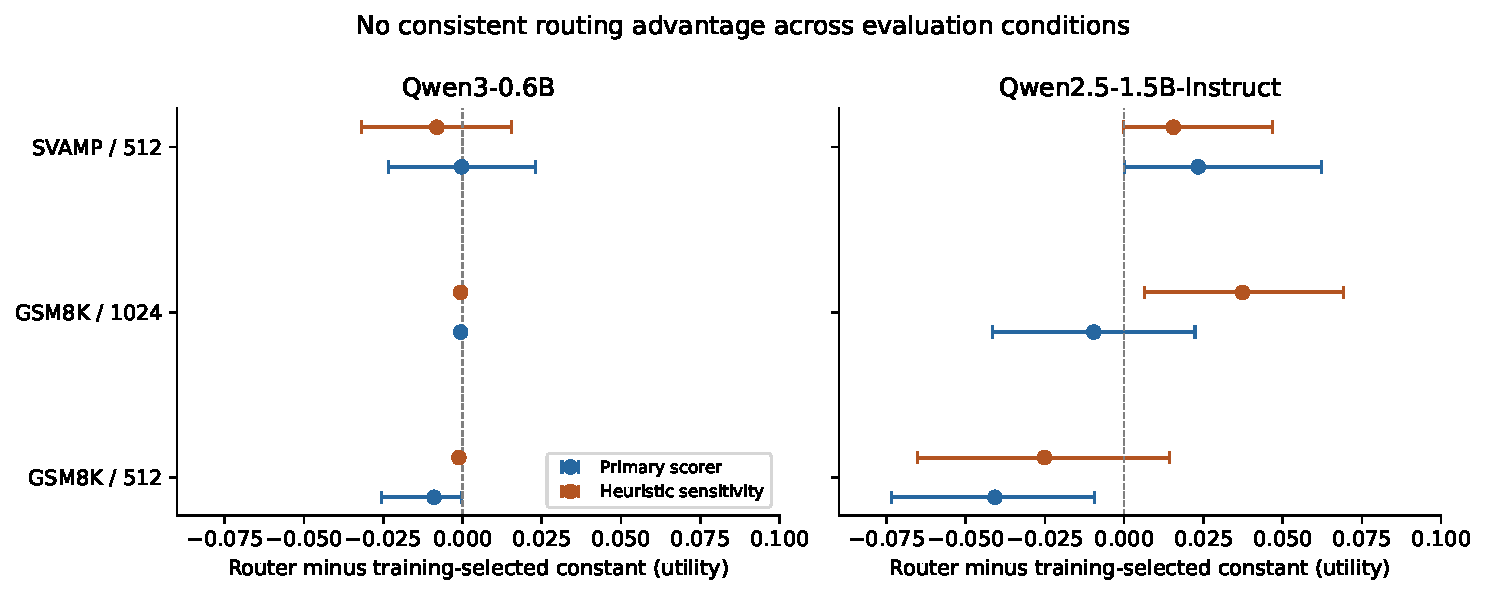
\includegraphics[width=\linewidth]{results.pdf}\caption{Same-policy contrasts under primary and sensitivity scoring; policies are not refitted on evaluation outcomes. Error bars are 95\% descriptive task-bootstrap intervals.}\label{fig:main}\end{figure}\section{Discussion and limitations}
The tested selector does not provide a consistent improvement over a training-selected constant. That result is useful as a baseline check: a question-dependent policy is not automatically better than a fixed workflow. It does not prove that adaptive selection cannot work. The lexical representation, small training set, and fixed candidate pool may constrain this particular policy.

The scoring discrepancy gives a second practical lesson. A workflow can improve compliance with an answer marker while changing the content of the answer differently. Evaluators should state the response contract and publish a separately specified sensitivity rather than select a favorable parser after seeing results. Our sensitivity is only a heuristic and can mistake a final unrelated number for an answer.

The two checkpoints are small and share a model family. Two seeds do not adequately characterize every stochastic behavior. Arithmetic transfer is narrow, public training contamination is possible, and no stronger embedding-based or bandit selector is implemented. The cost term omits input tokens and hardware variation from utility, although these quantities are separately recorded. It is not a money-saving estimate. Conditional bootstrap intervals omit training-sample uncertainty. Development selected the instruments before freezing, and their choice limits generalization.

\section{Responsible use}
These text-only workflows perform no external account actions. Their benchmark scores should not be used as deployment certifications or broad claims about autonomous systems. A related reliability study uses different primary tasks and interventions but shares software and ancestry; these are not independent replications. Historical AI-assisted validation is not independent human peer review.

\section{Conclusion}
The completed local evaluation offers no consistent selection advantage for this question-only ridge baseline. Its stronger lesson is methodological: retain the training-selected constant comparator, separate hindsight references from deployable policies, and make scorer-dependent conclusions visible. This is a bounded empirical finding rather than a new routing algorithm or a general ranking of multi-agent architectures.
\section*{Availability}\url{https://github.com/GouthamSiripuram/agent-architecture-selection}. This manuscript is a preprint; no arXiv identifier or peer-review acceptance is claimed.
\bibliography{references}
\bibliographystyle{tmlr}
\end{document}
